\documentclass[a4paper, twocolumn]{article}

\usepackage{colortbl}
\usepackage{cancel}
\usepackage{siunitx}
\usepackage{multirow}
\usepackage{array}
\usepackage[table, xcdraw, dvipsnames]{xcolor}
\usepackage{times}
\usepackage{tikz}
\usepackage[top=0.75in, bottom=1in, inner=0.75in, outer=0.75in,
            headheight=45pt, headsep=0in, footskip=0in]{geometry}
\usepackage{graphicx}
\usepackage{anyfontsize}
\usepackage{fancyhdr}
\usepackage{indentfirst}
\usepackage{amsmath}
\usepackage[spanish, es-tabla]{babel}
\usepackage[utf8]{inputenc}
\usepackage[explicit]{titlesec}
\usepackage{etoolbox}
\usepackage{enumitem}
\usepackage[labelformat=simple,labelsep=none]{caption}
\usepackage{mathptmx}
\usepackage{lastpage}
\usepackage{booktabs}
\usepackage{amsfonts}
\usepackage[version=4]{mhchem}
\usepackage{float}
\usepackage{circuitikz}
\usepackage{subcaption}
\usepackage[utf8]{inputenc}
\usepackage{changepage}
% \usepackage{showframe}

\include{newCommands}

\begin{document}
    \include{caratula}
    % \renewcommand{\normalsize}{\fontsize{12}{18}\selectfont}

\renewcommand{\headrulewidth}{0.4pt}
\renewcommand{\footrulewidth}{0.4pt}

\fancyhf{}
\fancyfoot[R]{[Parfait M. - Rao V. - Gatica M.] [\textbf{pág.\ \thepage} de \pageref{LastPage}]}
\definecolor{textoGris}{HTML}{222222}
\fancyhead[L]{
    \begin{tabular}{@{}l@{}}
        \raisebox{-0.5\height}{
\includegraphics[height=0.60in]{./imagenes/logoDepartamentoElectronica.png}}
        \begin{tabular}{@{}l@{}}
            {\color{textoGris}\textbf{Departamento de Ingeniería Electrónica}} \\
            {\color{textoGris}Facultad Regional Córdoba}
        \end{tabular}
    \end{tabular}
}

\titleformat{\section}[hang]{\fontsize{10}{12}\bfseries}{\thesection.}{0.5em}{\underline{#1}}
\titleformat{\subsection}[hang]{\fontsize{10}{11}\bfseries}{\thesubsection.}{0.5em}{#1}
\titleformat{\subsubsection}[hang]{\fontsize{10}{10}\itshape}{\thesubsubsection.}{0.5em}{#1}

\widowpenalty=10000
\clubpenalty=10000
\enlargethispage{-1cm}

    \thispagestyle{empty}
\setcounter{page}{0}
\clearpage
\onecolumn
\tableofcontents
\clearpage
\twocolumn
\newpage
\thispagestyle{empty}
\setcounter{page}{0}
\text{}
\newpage

    \saltoPag{}
    \section{Introducción}
\sangria{} En este trabajo práctico se analizaron diodos rectificadores y zener mediante simulaciones con LTspice y mediciones en laboratorio. Se evaluó su comportamiento en polarización directa e inversa, identificando parámetros clave como la tensión umbral y la zona de ruptura.

\sangria{} Se compararon diodos de silicio (1N4007) y germanio (1N60), utilizando herramientas como Python para graficar curvas I–V y contrastar con los datos experimentales. También se estudiaron aplicaciones prácticas, como circuitos recortadores con diodos zener, integrando conceptos fundamentales para el análisis y diseño de circuitos electrónicos.

\section{Preparación de las prácticas}
\sangria{} Temperatura ambiente del laboratorio al momento de hacer las actividades fue de $25^o$ celsius.
\imagen[Temperatura del laboratorio en ºC]{6cm}{./imagenes/temperaturaAmbiente.jpg}
\sangria{} A continuación se hará mención de los instrumentos de medición utilizados.
\imagen[Instrumentos de medición]{6cm}{./imagenes/instrumentosDeMedición.jpg}
1) \underline{Multímetro}
\begin{itemize}
    \item \textbf{Fabricante:} Pro'sKit
    \item \textbf{Modelo:} MT-1706 CAT 1000V
    \item \textbf{Serie:} MT-17XX
\end{itemize}
\begin{center}
    \begin{tabular}{| p{1cm}  p{1cm}  |}
        \hline
        \multicolumn{2}{|c|}{\textbf{Información de mediciones}} \\
        \hline
        \multicolumn{1}{|m{4cm}}{\centering\textbf{Tensión CC} \\ 60V - Res: 10mV} &
        \multicolumn{1}{|m{3cm}|}{\centering$\pm 0,5\%$ \\+ $3$ dig.} \\
        \hline
        \multicolumn{1}{|m{4cm}}{\centering\textbf{Temperatura $[^oC]$} \\ -20 a 1000$^oC$ - Res: $1^oC$} &
        \multicolumn{1}{|m{3cm}|}{\centering$\pm1,0\% lectura$ \\+ $3$ dig.} \\
        \hline
        \multicolumn{1}{|m{3cm}}{\centering\textbf{Resistencia} \\ $60k\Omega$ - Res: $10\Omega$} &
        \multicolumn{1}{|m{3cm}|}{\centering$\pm 0,8\%$ lectura \\+ $3$ dig.} \\
        \hline
    \end{tabular}
\end{center}

2) \underline{Osciloscopio - multímetro - generador de señales}
\begin{itemize}
    \item \textbf{Fabricante:} FNIRSI
    \item \textbf{Modelo:} 2C23T
    \item \textbf{Serie:} ---
\end{itemize}
\begin{center}
    \begin{tabular}{| p{1cm}  p{1cm}  |}
        \hline
        \multicolumn{2}{|c|}{\textbf{Información de mediciones}} \\
        \hline
        \multicolumn{1}{|m{4cm}}{\centering\textbf{Corriente CC} \\ auto-rango} &
        \multicolumn{1}{|m{3cm}|}{\centering$9999\mu A \rightarrow 9,999A \pm (1,2\%+3)$} \\
        \hline
    \end{tabular}
\end{center}

3) \underline{Multímetro}
\begin{itemize}
    \item \textbf{Fabricante:} BRYMEN
    \item \textbf{Modelo:} BM857S
    \item \textbf{Serie:} BM850A DMM Series
\end{itemize}
\begin{center}
    \begin{tabular}{| p{1cm}  p{1cm}  |}
        \hline
        \multicolumn{2}{|c|}{\textbf{Información de mediciones (modo multímetro)}} \\
        \hline
        \multicolumn{1}{|m{4cm}}{\centering\textbf{Tensión CC} \\ auto-rango} &
        \multicolumn{1}{|m{3cm}|}{$\centering 500mV \rightarrow 50V \pm 0,03\% 2+d$} \\
        \hline
    \end{tabular}
\end{center}

4) \underline{Fuente de tensión continua de la facultad F-44}
\imagen{7cm}{./imagenes/fuenteDeDudosaCalidad.jpg}

\section{Actividad de laboratorio I}
 El objetivo de esta actividad ha sido el de identificar los terminales de los diodos, la comprobación de su correcto funcionamiento y la obtención de la tensión umbral de polarización.
\newpage
 \midTitle{red}{Materiales utilizados}
 \begin{itemize}[noitemsep]
    \item Dos diodos de silicio 1N4007 y otros dos de germanio 1N60. \\
    \begin{center} \diodoSilicio{1N4007} \diodoGermanio{1N60} \end{center}
    \item Multímetro.
    \item Protoboard.
\end{itemize}
\subsection{Identificación de pines y funcionamiento de diodos}
\sangria{} Se colocó el multímetro en modo detección de diodo (mismo que se usa para la continuidad).
\sangria{} Se colocó los diodos en la protoboard, y se procedió a medir los terminales de estos en un sentido y otro.


\begin{center}
    \tikzset{
          hole/.style = {fill = #1, circle, minimum width = 1mm, inner sep = 0mm},
          wire/.style = {draw = #1, line width = 0.2mm},
          label/.style = {rotate = 0, black!50!white, font=\sffamily, anchor = center}
        }
        \begin{tikzpicture}[x=2mm,y=2mm]
          \draw[fill=black!05!white] (-4,-1) rectangle (16,34);
 
          \foreach \yi in {1,...,30}{
            \node[hole=red]  at (-3,\yi){};
            \node[hole=blue] at (-2,\yi){};
            \node[hole=red]  at (14,\yi){};
            \node[hole=blue] at (15,\yi){};

            \foreach \xs in {0,6}{
                \foreach \xi in {1,2,3,4,5}{
                    \node[hole=black] at (\xi+\xs,\yi){};
                }
            }
        }

        \foreach \m/\xi in {A/1,B/2,C/3,D/4,E/5,F/7,G/8,H/9,I/10,J/11}{
            \node[label=0] at (\xi, 0) {\tiny\m};
            \node[label=0] at (\xi,31) {\tiny\m};
        }

        \foreach \n/\yi in {1,5,10,15,20,25,30}{
            \node[label=0] at (-1,\yi) {\tiny\n};
            \node[label=0] at (13,\yi) {\tiny\n};
        }  
        \filldraw[fill=white, draw=black] (4.5, 26) rectangle (5.5, 29);
        \fill[fill=orange!80] (4.75, 28) rectangle (5.25, 26);
        \draw[line width=1pt, draw=gray!80] (5, 29) -- (5, 30);
        \draw[line width=1pt, draw=gray!80] (5, 26) -- (5, 25);
        \fill[fill=gray!95] (4.5, 28) rectangle (5.5, 29);

        \filldraw[fill=white, draw=black] (3.5, 24) rectangle (4.5, 27);
        \fill[fill=orange!80] (3.75, 27) rectangle (4.25, 24);
        \draw[line width=1pt, draw=gray!80] (4, 27) -- (4, 28);
        \draw[line width=1pt, draw=gray!80] (4, 24) -- (4, 23);
        \fill[fill=gray!95] (3.5, 26) rectangle (4.5, 27);

        \filldraw[fill=black!75, draw=black] (2.5, 22) rectangle (3.5, 24.5);
        \draw[line width=1pt, draw=gray!80] (3, 24.5) -- (3, 26);
        \draw[line width=1pt, draw=gray!80] (3, 22) -- (3, 21);
        \fill[fill=gray!95] (2.5, 22.5) rectangle (3.5, 23);

        \filldraw[fill=black!75, draw=black] (1.5, 20) rectangle (2.5, 22.5);
        \draw[line width=1pt, draw=gray!80] (2, 22.5) -- (2, 24);
        \draw[line width=1pt, draw=gray!80] (2, 20) -- (2, 19);
        \fill[fill=gray!95] (1.5, 20.5) rectangle (2.5, 21);

        \draw[-latex, very thick, orange, line width=0.75mm] (-15, 20.5) -- (-9, 20.5) -- (1, 20.5);
        \node[anchor=west] at (-15, 22) {\Large 1N4007};

        \draw[-latex, very thick, violet, line width=0.75mm] (25,26) -- (6,26);
        \node[anchor=east] at (25,27.5) {\Large 1N60};

    \end{tikzpicture}
\end{center}

\imagen[Disposición de diodos]{7cm}{./imagenes/disposicionDeDiodos.jpg}

\subsubsection{Valores con el diodo 1N60}
\imagen[Medición en directa]{7cm}{./imagenes/medicionDirecta1N60.jpg}
\imagen[Valores del multímetro en p. directa]{7cm}{./imagenes/medicionDirecta1N60Multimetro.jpg}
\imagen[Medición en inversa]{7cm}{./imagenes/medicionInversa1N60.jpg}
\imagen[Valores del multímetro en p. inversa]{7cm}{./imagenes/medicionInversa1N60Multimetro.jpg}

\begin{center}
\begin{table}[]
    \begin{tabular}{|p{2cm}|p{0.8cm}p{0.9cm}|p{0.8cm}p{0.9cm}|}
\hline
\cellcolor[HTML]{FFFC9E}                                                                                                              & \multicolumn{2}{c|}{\cellcolor[HTML]{FFFFC7}\textbf{1N60}} & \multicolumn{2}{c|}{\cellcolor[HTML]{FF9390}\textbf{1N4007}} \\ \cline{2-5} 
\multirow{-2}{*}{\cellcolor[HTML]{FFFC9E}\textbf{\begin{tabular}[c]{@{}c@{}}Sentido de las \\ puntas del \\ multímetro\end{tabular}}} & \multicolumn{1}{c|}{\textbf{D1}}        & \textbf{D2}        & \multicolumn{1}{c|}{\textbf{D1}}       & \textbf{D2}       \\[12pt] \hline
\begin{tabular}[c]{@{}c@{}}Polarización \\ directa\end{tabular}                                                                       & \multicolumn{1}{c|}{0,373V}             & 0,401V             & \multicolumn{1}{c|}{0,593V}            & 0,614V            \\ \hline
\begin{tabular}[c]{@{}c@{}}Polarización \\ inversa\end{tabular}                                                                       & \multicolumn{1}{c|}{0V}                 & 0V                 & \multicolumn{1}{c|}{0V}                & 0V                \\ \hline
\end{tabular}
\end{table}
\end{center}

\begin{figure}[H]
    \centering
    \begin{subfigure}[b]{0.45\linewidth}
        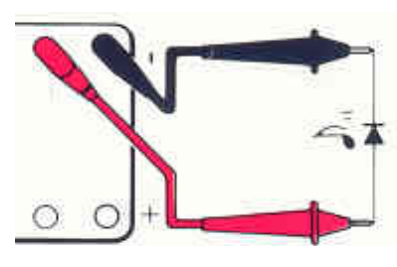
\includegraphics[width=3.5cm]{./imagenes/polarizacionDirecta.png}
        \caption{Polarización Directa}
    \end{subfigure}
    \hfill
    \begin{subfigure}[b]{0.45\linewidth}
        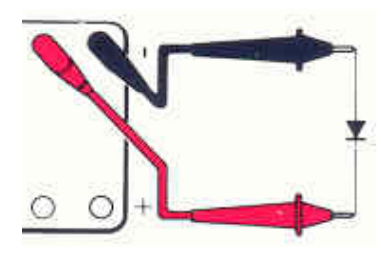
\includegraphics[width=3.5cm]{./imagenes/polarizacionInversa.png}
        \caption{Polarización Inversa}
    \end{subfigure}
    \caption{Modos de polarización del diodo}
    \label{fig:polarizaciones}
\end{figure}

\subsection{Conclusión de la identificación de pines}
\sangria{} Se identificaron correctamente los terminales de los diodos 1N4007 y 1N60 utilizando el multímetro en modo de prueba de diodos. Se verificó que, al aplicar la polarización directa, los diodos condujeron corriente mostrando una caída de tensión en el rango esperable para cada tecnología: aproximadamente 0,6V para el 1N4007 (silicio) y entre 0,37V y 0,4V para el 1N60 (germanio).

\sangria{} En polarización inversa, ambos diodos bloquearon el paso de corriente, como se esperaba, indicando que no presentaban fallas internas. A partir de estas pruebas simples pero efectivas, se lograron identificar el ánodo y el cátodo en cada diodo, permitiendo su correcta utilización.


    \section{Actividad de laboratorio II}

\sangria{} El objetivo de esta actividad es medir las corrientes y tensiones de los diodos rectificadores, tanto los de silicio como los de germanio. Posteriormente se comparará los resultados con los datasheet de estos diodos.

\subsection{Actividad de simulación}

\sangria{} Para esta actividad se analizó el momento en el que un dispositivo pasa del estado de bloqueo a conducción, usando el simulador LTspice.\\

\textbf{Nota:} el simulador LTspice no posee el diodo 1N60 \\ en su menú de dispositivos, por lo que hemos decidido escribir nuestro diodo 1N60 usando de base su datasheet:

\begin{quote}
    \ttfamily
    .MODEL 1N60 D(IS=0.1E-3 BV=40 RS=1.0 CJO=2.0E-12 N=1.5 VJ=0.32 M=0.5 TT=1E-9)
\end{quote}

Siendo:
\begin{itemize}[noitemsep, topsep = 0pt]
    \item \textbf{IS}: Corriente de saturación inversa.
    \item \textbf{BV}: Tensión de ruptura inversa.
    \item \textbf{RS}: Resistencia serie.
    \item \textbf{CJO}: Capacitancia de unión en polarización cero.
    \item \textbf{N}: Coeficiente de idealidad.
    \item \textbf{VJ}: Tensión de juntura.
    \item \textbf{M}: Coeficiente de gradiente de la unión.
    \item \textbf{TT}: Tiempo de recuperación.
\end{itemize}
\subsubsection{Polarización en directa}
\sangria{} En este inciso se analizó la polarización en directa de los diodos 1N4007 y 1N60 por medio del siguiente circuito:

\imagen[Circuito de prueba con d. 1N4007, para el 1N60 se implementó un circuito similar]{8cm}{./imagenes/circuitoLtspice1N4007.png}

\sangria{} El entorno de simulación fue configurado para hacer un barrido de la fuente V1 (la celda de tensión continua), comenzando desde -2V a 10V con un paso de 100mV para cada muestreo.

\imagen[Configuración de la simulación]{7cm}{./imagenes/configuracionEntornoLtspice1N4007.png}
\newpage\thispagestyle{fancy}
\textbf{Resultados:}

\sangria{} Se obtuvo la gráfica de la corriente del diodo en función de su tensión ($I_{D1}$). 

\imagen[Curva del diodo 1N4007]{7cm}{./imagenes/graficoCorrienteVSTension1N4007.png}

\imagen[Curva del diodo 1N34A]{7cm}{./imagenes/graficoCorrienteVSTension1N60.png}

\inicioCodigo{}

\subsubsection{Curvas en Python}

\begin{minted}{python}
import pandas as pd 
import matplotlib.pyplot as plt 

df4007 = pd.read_csv("simulacionDiodo1N4007.txt", sep="\t")
df4007.columns = ["Voltaje (V)", "Corriente (A)"]
df60 = pd.read_csv("simulacionDiodo1N60.txt", sep="\t")
df60.columns = ["Voltaje (V)", "Corriente (A)"]
plt.figure(figsize=(10, 6))
plt.plot(df4007["Voltaje (V)"], df4007["Corriente (A)"], label="1N4007", color="red")
plt.plot(df60["Voltaje (V)"], df60["Corriente (A)"], label="1N60", color="blue")
plt.axhline(0, color='black', linewidth=0.5)
plt.axvline(0, color='black', linewidth=0.5)
plt.title("Curva I-V del diodo 1N4007 y 1N60")
plt.xlabel("Voltaje [V]")
plt.ylabel("Corriente [A]")
plt.legend()
plt.tight_layout()
plt.savefig("graficoCorrienteVSTensionDiodosPython.png")
\end{minted}

\imagen[Output]{15cm}{./imagenes/graficoCorrienteVSTensionDiodosPython.png}

\finalCodigo{}

\subsubsection{Polarización en inversa}
\sangria{} En este inciso se pondrá los diodos en polarización inversa, usando de base el circuito anteriormente mencionado. \\
\sangria{} Se sabe que los diodos tienen una funcionalidad de ponerse en "bloque" (no conduce la corriente) cuando el cátodo tiene mayor potencial que el ánodo. Se hizo la simulación con el objetivo de superar la tensión de ruptura del diodo y provocar una avalancha de corriente en polarización inversa. 

\sangria{} Conocer la tensión de ruptura del diodo implica revisar las hojas de datos del diodo 1N4007 y 1N60:
\begin{center}
    \begin{tabular}{|c|l|l|}
    \rowcolor[HTML]{FFCE93}
    \hline
    \textbf{Diodo} & 
    \multicolumn{1}{c|}{\cellcolor[HTML]{FFCE93}\textbf{Tensión ruptura}} & 
    \multicolumn{1}{c}{\cellcolor[HTML]{FFCE93}{\color[HTML]{000000} \textbf{Fabricante}}} 
    \\ 
    \hline
    \cellcolor[HTML]{FFFC9E}{\color[HTML]{000000} \textbf{1N60}} &
    40v &
    DEC \\
    \hline 
    \cellcolor[HTML]{FFFC9E}\textbf{1N4007} &
    1000v & 
    Taiwan s.c. \\ 
    \hline
    \end{tabular}
\end{center}

\begin{center} \textit{Datasheet's en la bibliografía} \end{center}

\sangria{} Para la simulación, se configuró el barrido para que cada diodo llegue a su tensión de ruptura en inversa agregando más tensión de lo que el fabricante menciona. Por lo que al diodo 1N4007 se le agregó un barrido a 1100V y al diodo 1N60, 50V. Además, se configuró el LTspice para empezar desde -10V, con estos valores podemos ver que comienza el barrido con el diodo en polarización directa, se pasa a polarización inversa y luego alcanza la tensión de ruptura.

\imagen[Diodo 1N60 polarizado en inversa, el 1N4007 es similar]{7cm}{./imagenes/circuitoLtspice1N60Inversa.png}

\imagen[Configuración del barrido en LTspice]{8cm}{./imagenes/configuracionEntornoLtspice1N60Inversa.png}

\imagen[Gráfico I-V diodo 1N60 en inversa]{8cm}{./imagenes/graficoCorrienteVSTension1N60Inversa.png}

\imagen[Gráfico I-V diodo 1N4007 en inversa]{8cm}{./imagenes/graficoCorrienteVSTension1N4007Inversa.png}

\inicioCodigo{}
\subsubsection{Curvas en Python}

\begin{minted}{python}
import pandas as pd 
import matplotlib.pyplot as plt 

df4007 = pd.read_csv("simulacionDiodo1N4007Inversa.txt", sep="\t")
df4007.columns = ["Voltaje (V)", "Corriente (A)"]
df60 = pd.read_csv("simulacionDiodo1N60Inversa.txt", sep="\t")
df60.columns = ["Voltaje (V)", "Corriente (A)"]
plt.figure(figsize=(10, 6))
plt.plot(df4007["Voltaje (V)"], df4007["Corriente (A)"], label="1N4007", color="red")
plt.plot(df60["Voltaje (V)"], df60["Corriente (A)"], label="1N60", color="blue")
plt.axhline(0, color='black', linewidth=0.5)
plt.axvline(0, color='black', linewidth=0.5)
plt.title("Curva I-V del diodo 1N4007 y 1N60")
plt.xlabel("Voltaje [V]")
plt.ylabel("Corriente [A]")
plt.legend()
plt.tight_layout()
plt.savefig("graficoCorrienteVSTensionDiodosInversaPython.png")
\end{minted}

\imagen[Output]{15cm}{./imagenes/graficoCorrienteVSTensionDiodosInversaPython.png}

\finalCodigo{}

\subsubsection{Conclusión de las simulaciones}
\sangria{} Las simulaciones realizadas en LTspice permitieron analizar el comportamiento de los diodos 1N4007 y 1N60 tanto en polarización directa como en inversa. En polarización directa se pudo observar cómo el diodo de germanio (1N60) comienza a conducir a un voltaje más bajo que el de silicio (1N4007), mostrando una menor tensión umbral, coherente con lo esperado por la tecnología de fabricación.

\sangria{} En polarización inversa, los resultados mostraron que ambos diodos permanecen en bloqueo hasta alcanzar su tensión de ruptura. El 1N60 mostró ruptura alrededor de los 40V, mientras que el 1N4007 la alcanzó cerca de los 1000V, lo cual coincide con los valores extraídos de los datasheets.

\sangria{} Estas simulaciones, complementadas con modelos SPICE realistas y gráficos obtenidos mediante Python, brindan una representación clara y visual del funcionamiento de los diodos ante distintas condiciones de polarización.

\subsection{Curva característica de los diodos}

\sangria{} En esta sección se realizó de manera práctica lo visto en las simulaciones del punto anterior (excepto el relevamiento de la zona de ruptura inversa). \\
\sangria{} Lo que se buscó fue reconocer el comportamiento no ideal de los diodos y encontrar un ''codo'': la parte del gráfico del diodo donde comienza a conducir corriente en polarización directa.

\imagen[Circuito propuesto]{8cm}{./imagenes/circuitoPropuestoCurvasDiodo.png}
\begin{center}
    \tikzset{
          hole/.style = {fill = #1, circle, minimum width = 1mm, inner sep = 0mm},
          wire/.style = {draw = #1, line width = 0.2mm},
          label/.style = {rotate = 0, black!50!white, font=\sffamily, anchor = center}
        }
        \begin{tikzpicture}[x=2mm,y=2mm]
          \draw[fill=black!05!white] (-4,-1) rectangle (16,34);
 
          \foreach \yi in {1,...,30}{
            \node[hole=red]  at (-3,\yi){};
            \node[hole=blue] at (-2,\yi){};
            \node[hole=red]  at (14,\yi){};
            \node[hole=blue] at (15,\yi){};

            \foreach \xs in {0,6}{
                \foreach \xi in {1,2,3,4,5}{
                    \node[hole=black] at (\xi+\xs,\yi){};
                }
            }
        }

        \foreach \m/\xi in {A/1,B/2,C/3,D/4,E/5,F/7,G/8,H/9,I/10,J/11}{
            \node[label=0] at (\xi, 0) {\tiny\m};
            \node[label=0] at (\xi,31) {\tiny\m};
        }

        \foreach \n/\yi in {1,5,10,15,20,25,30}{
            \node[label=0] at (-1,\yi) {\tiny\n};
            \node[label=0] at (13,\yi) {\tiny\n};
        }

        \filldraw[fill=black!75, draw=black] (-1, 20.5) rectangle (1.5, 21.5);
        \draw[line width=1pt, draw=gray!80] (-2, 21) -- (-1, 21);
        \draw[line width=1pt, draw=gray!80] (1.5, 21) -- (3, 21);
        \fill[fill=gray!95] (-0.5, 20.5) rectangle (0, 21.5);

        \filldraw[fill=brown!60, draw=black] (4.5, 22.5) rectangle (5.5, 25);
        \draw[line width=1pt, draw=gray!80] (5, 22.5) -- (5, 21);
        \draw[line width=1pt, draw=gray!80] (5, 25) -- (5, 27);
        \fill[fill=brown] (4.5, 22.75) rectangle (5.5, 23);
        \fill[fill=black] (4.5, 23.25) rectangle (5.5, 23.5);
        \fill[fill=red] (4.5, 23.75) rectangle (5.5, 24);
        \fill[fill=gold] (4.5, 24.25) rectangle (5.5, 24.5);

        \draw[line width=1.5pt, draw=black!90] (-6, 25) -- (-6, 40) -- (-4.20,40);
        \draw[line width=1.5pt, draw=red!90] (4, 27) -- (4, 40) -- (-2.3, 40);
        \filldraw[line width=1.5pt, fill=orange!25] (-1, 40) circle (0.60cm);
        \filldraw[draw=black!90] (-4.25,40) circle (2pt);
        \filldraw[draw=black!90] (2.25,40) circle (2pt);
        \node at (1, 40) {\large\textbf{+}};
        \node at (-3, 39.85) {\large\textbf{-}};
        \node at (13, 49) {\Large\textbf{$V_{CC}$}};

        \filldraw[line width=1.25pt, fill=Aquamarine, draw=black, thick]
            (8, 41) -- (9, 41) -- (9.25, 41.25) -- (11.75, 41.25) -- (12, 41)
            -- (18, 41) -- (18, 46) -- (12, 46) -- (11.75, 45.75) -- 
            (9.25, 45.75) -- (9, 46) -- (8, 46) -- cycle;

        \filldraw[line width=0.75pt, fill=black!50, draw=black!90] (10.5, 43.5) circle (8pt);
        \filldraw[line width=0.75pt, fill=blue!30, draw=black!90] (14, 41.25) rectangle (17.5, 45.75);

        \draw[line width=1.5pt, draw=red!80] (4, 40) -- (4, 42) -- (8.5, 42);
        \draw[line width=1.5pt, draw=black!80] (-6, 40) -- (-6, 46) -- (4, 46) -- (4, 43) -- (8.5, 43);
        
        \filldraw[line width=0.75pt, fill=blue!60, draw=black!90] (-7.5, 20.5) rectangle (-10, 26.5);
        \filldraw[line width=0.75pt, fill=blue!60, draw=black!90] (-13.6, 20.5) rectangle (-16.5, 26.5);

        \filldraw[line width=1.5pt, draw=black!90, fill=black!85] ( -8, 26) rectangle (-16, 21);
        \filldraw[line width=0.75pt, draw=black!90, fill=pink!20] (-13, 21.25) rectangle (-15.5, 25.75);

        \draw[line width=1.5pt, draw=black!90] (-6, 25) -- (-9, 25);
        \draw[line width=1.5pt, draw=black!90] (-9, 24) -- (-6, 24) -- (-6, 22) -- (-1.75, 22);

        \node at (-12, 30) {\Large\textbf{$I_D$}};

        \filldraw[line width=1.5pt, draw=black!90, fill=red!70] (-6.5, 13.5) rectangle (-17.5, 7.5); 
        \filldraw[line width=1.5pt, draw=black!90, fill=black!70] (-7, 13) rectangle (-17, 8);
        \draw[line width=1.5pt, draw=black!90] (-8, 12) -- (-1.25, 12) -- (-1.25, 21);
        \draw[line width=1.5pt, draw=red!80] (-8, 11) -- (2, 11) -- (2, 21);

        \filldraw[line width=0.75pt, draw=black!90, fill=blue!30] (-14, 12.5) rectangle (-16.5, 8.5);
        \filldraw[draw=black!90, fill=black!75, line width=0.75pt] (-12, 10.5) circle (8pt);

        \node at (-12, 16) {\Large\textbf{$V_D$}};

        \draw[-latex, very thick, draw=orange, line width=0.75mm] (23, 35) -- (11, 35) -- (9, 23.75) -- (6, 23.75);
        \node[anchor=east] at (22,37) {\Large $1K\Omega$ \small $1/4w$};

    \end{tikzpicture}
\end{center}

\imagen[]{8cm}{./imagenes/circuitoCurvasCaracteriscaDiodo.jpg}

El procedimiento de este ensayo fue el siguiente:
\begin{enumerate}
    \item   Una vez armado el circuito, se partió midiendo el voltaje y corriente del diodo limitado por la resistencia.
    \item   Se arrancó con 0v de la fuente $V_{CC}$, se tomó nota de los valores del diodo y luego se siguió aumentando el voltaje de la fuente hasta los 5v, tomando muestras de por medio.
    \item   Se hizo lo mismo tanto para el diodo 1N4007 (silicio) y el 1N60 (germanio).
\end{enumerate}

\sangria{} Este circuito nos permitió obtener valores de tensión - corriente del diodo para luego graficarlos y visualizar una curva del diodo ''más realista'' que las obtenidas por la simulación con LTspice.
\midTitle{red}{\textbf{Valores - Diodo 1N4007}}
\thispagestyle{fancy}

\begin{center}
    \renewcommand{\arraystretch}{1.25}
    \begin{tabular}{|c|c|c|c|c|c|c|}
    \hline
    \rowcolor[HTML]{FFFFC7} 
    $V_1 [V]$                              & 0   & 0,1 & 0,3 & 0,4 & 0,45 & 0,5 \\ \hline
    \cellcolor[HTML]{FFFC9E}$V_D$ {[}mV{]} & 7,7 & 101 & 294 & 394 & 427  & 459 \\ \hline
    \cellcolor[HTML]{FFCE93}$I_D$ {[}mA{]} & -3  & -4  & -4  & 1   & 10   & 35  \\ \hline
    \end{tabular}
    \par\vspace{10pt}\par
    \small
    \begin{tabular}{|c|c|lc|c|c|c|c|}
    \hline
    \rowcolor[HTML]{FFFFC7} 
    $V_1 [V]$                              & 0,55 & \multicolumn{1}{l|}{\cellcolor[HTML]{FFFFC7}0,6} & 0,65 & 0,7 & 1   & 3    & 5    \\ \hline
    \cellcolor[HTML]{FFFC9E}$V_D$ {[}mV{]} & 480  & 498                                              & 512  & 523 & 563 & 643  & 672  \\ \hline
    \cellcolor[HTML]{FFCE93}$I_D$ {[}mA{]} & 52   & 75                                               & 110  & 130 & 345 & 1335 & 4435 \\ \hline
    \end{tabular}
\end{center}

\midTitle{blue}{\textbf{Valores - Diodo 1N60}}

\begin{center}
    \renewcommand{\arraystretch}{1.25}
    \begin{tabular}{|c|c|c|c|c|c|c|}
    \hline
    \rowcolor[HTML]{FFFFC7} 
    $V_1 [V]$                              & 0  & 0,1 & 0,3 & 0,4 & 0,45 & 0,5 \\ \hline
    \cellcolor[HTML]{FFFC9E}$V_D$ {[}mV{]} & 6  & 75  & 162 & 184 & 196  & 202 \\ \hline
    \cellcolor[HTML]{FFCE93}$I_D$ {[}mA{]} & -4 & 22  & 135 & 207 & 252  & 275 \\ \hline
    \end{tabular}
    \par\vspace{10pt}\par
    \small
    \begin{tabular}{|c|c|lc|c|c|c|c|}
    \hline
    \rowcolor[HTML]{FFFFC7} 
    $V_1 [V]$                              & 0,55 & \multicolumn{1}{l|}{\cellcolor[HTML]{FFFFC7}0,6} & 0,65 & 0,7 & 1   & 3    & 5    \\ \hline
    \cellcolor[HTML]{FFFC9E}$V_D$ {[}mV{]} & 216  & 225                                              & 231  & 241 & 286 & 475  & 655  \\ \hline
    \cellcolor[HTML]{FFCE93}$I_D$ {[}mA{]} & 333  & 371                                              & 410  & 458 & 724 & 2512 & 4355 \\ \hline
    \end{tabular}
\end{center}

\subsubsection{Conclusiones de las curvas}
\sangria{} A partir de las curvas características obtenidas de manera experimental, se confirmó el comportamiento teórico de ambos diodos. El 1N60 mostró conducción a partir de una menor tensión en directa (aproximadamente 0,2V – 0,3V), lo que se refleja en una pendiente más suave y una mayor corriente en las primeras etapas del gráfico. Por el contrario, el 1N4007, al ser de silicio, mostró una tensión umbral más alta, cercana a los 0,6V, con una región de no conducción más extensa.

\sangria{} La relación entre la corriente y la tensión medida permitió identificar claramente el ''codo'' característico del diodo en polarización directa. Además, los valores obtenidos muestran buena correlación con los resultados de las simulaciones, validando tanto el montaje como el procedimiento experimental.

\sangria{} En conjunto, los resultados demuestran de forma clara las diferencias prácticas entre diodos de silicio y germanio, y cómo esas diferencias impactan en su aplicación dentro de circuitos electrónicos reales.

\inicioCodigo{}
\subsubsection{Curvas en Python}

\begin{minted}{python}
import matplotlib.pyplot as plt

voltajeFuente = [0, 0.1, 0.3, 0.4, 0.45, 0.5, 0.55, 0.6, 0.65, 0.7, 1, 3, 5]

voltajeDiodo1N4007 = [7.7, 101, 294, 394, 427, 459, 480, 498, 512, 523, 563, 643, 672]
corrienteDiodo1N4007 = [-3, -4, -4, 1, 10, 35, 52, 75, 110, 130, 345, 1335, 4435]

voltajeDiodo1N60 = [6, 75, 162, 184, 196, 202, 216, 225, 231, 241, 286, 475, 655]
corrienteDiodo1N60 = [-4, 22, 135, 207, 252, 275, 333, 371, 410, 458, 724, 2512, 4355]

voltajeDiodo1N4007 = [v / 1000 for v in voltajeDiodo1N4007]
voltajeDiodo1N60 = [v / 1000 for v in voltajeDiodo1N60]

plt.figure(figsize=(10, 5))
plt.subplot(1, 2, 1)
plt.plot(voltajeFuente, corrienteDiodo1N4007, marker='o', color='red', label='1N4007')
plt.plot(voltajeFuente, corrienteDiodo1N60, marker='s', color='blue', label='1N60')
plt.title('Corriente vs Voltaje Fuente')
plt.xlabel('Voltaje de la Fuente [V]')
plt.ylabel('Corriente $I_D$ [mA]')
plt.legend()

plt.subplot(1, 2, 2)
plt.plot(voltajeFuente, voltajeDiodo1N4007, marker='o', color='red', label='1N4007')
plt.plot(voltajeFuente, voltajeDiodo1N60, marker='s', color='blue', label='1N60')
plt.title('Voltaje del Diodo vs Voltaje Fuente')
plt.xlabel('Voltaje de la Fuente [V]')
plt.ylabel('Voltaje en el Diodo $V_D$ [V]')
plt.legend()

plt.tight_layout()
plt.savefig("graficosValoresRealesDiodos.png")

\end{minted}

\imagen[Output]{15cm}{./imagenes/graficosValoresRealesDiodos.png}

\finalCodigo{}

    \section{Actividad de laboratorio III}

	\subsection{Actividad de simulación: coportamiento del diodo en función de la temperatura}
	\sangria{} Circuito de simulación

	\begin{tikzpicture}
	% Paths, nodes and wires:
	\draw (2, 5.25) -- (3.25, 5.25);
	\draw (2, 3) -- (3.25, 3);
	\draw (-0.25, 5.25) to[american resistor] (1, 5.25);
	\draw (1, 5.25) -- (2, 5.25);
	\draw (-1, 4.404) to[american voltage source] (-1, 3.604);
	\draw (2, 3) -- (-1, 3) -| (-1, 3.6);
	\draw (-0.25, 5.25) -| (-1, 4.404);
	\draw (3.259, 4.4) to[full diode] (3.259, 4);
	\draw (3.259, 4.4) |- (3.109, 5.25);
	\draw (3.259, 4) |- (3.109, 3);
	\end{tikzpicture}

		\subsubsection{Conclusiones del cambio de temperatura}
		\sangria{} Podemos observar como a un aumento de temeperatura $20 \degree C$, $100 \degree C$, $125 \degree C $, aumenta la corriente de conducción para un  mismo voltaje aplicado en polarización directa. Esto se debe a que al incrementarse la temperatura, disminuye la barrera de potencial interna en el diodo (tensión umbral), facilitando el paso de la corriente.La corriente en la región de conducción directa se ve intensificada lo que sugiere una menor resistencia en el diodo, el aumento de la temeperatura también afecta a la corriente de fuga en polarización inversa, ya que al aumentar las temeperatura aumenta la generación de portadores minoritarios.
		\sangria{} Podemos concluir que la conductividad del diodo aumenta, pero sus parámetros electricos se vuelven menos precisos, afectando su funcionamiento en aplicaciones reales.

	\subsection{Actividad de simulación:circuitos recortadores con diodos zener}
		\subsubsection{Pequeña introducción a los diodos como recortadores}
		\sangria Para obtener el máximo valor de salida en el circuito se cumple que en cada semiciclo la tensión de recorte es igual a la tensión del diodo en directa $\approx 0,7V$ más la tensión de ruptura del diodo zener en inversa $V_{z}$, esta relación se va a cumplir tanto para el

		\begin{equation}
			V_{recorte}= V_{z} + 0,7V
		\end{equation}
    \sangria{} \textbf{Circuito A}

\begin{tikzpicture}
	% Paths, nodes and wires:
	\draw (2, 4.966) to[full ZZener diode] (2, 4.716);
	\draw (2, 3.213) to[full ZZener diode] (2, 3.663);
	\draw (2, 4.75) -| (2, 3);
	\draw (2, 5.25) -- (3.25, 5.25);
	\draw (2, 3) -- (3.25, 3);
	\draw (-0.991, 3.634) to[sinusoidal current source] (-0.991, 4.384);
	\draw (-0.25, 5.25) to[american resistor] (1, 5.25);
	\draw (-0.991, 4.384) |- (-0.25, 5.25);
	\draw (1, 5.25) -- (2, 5.25);
	\draw (-0.991, 3.634) |- (2, 3);
	\node[shape=rectangle, draw, line width=1pt, inner sep=0, minimum width=-0.035cm, minimum height=-0.035cm] at (3, 4.75){};
	\draw (2, 5.25) -| (2, 5);
	\end{tikzpicture}

	\sangria{} \textbf{Circuito B}

	\begin{tikzpicture}
	% Paths, nodes and wires:
	\draw (2, 4.5) to[full ZZener diode] (2, 5);
	\draw (2, 4) to[full ZZener diode] (2, 3.25);
	\draw (2, 4.75) -| (2, 3);
	\draw (2, 5.25) -- (3.25, 5.25);
	\draw (2, 3) -- (3.25, 3);
	\draw (-0.991, 3.634) to[sinusoidal current source] (-0.991, 4.384);
	\draw (-0.25, 5.25) to[american resistor] (1, 5.25);
	\draw (-0.991, 4.384) |- (-0.25, 5.25);
	\draw (1, 5.25) -- (2, 5.25);
	\draw (-0.991, 3.634) |- (2, 3);
	\node[shape=rectangle, draw, line width=1pt, inner sep=0, minimum width=-0.035cm, minimum height=-0.035cm] at (3, 4.75){};
	\draw (2, 5.25) -| (2, 5);
	\end{tikzpicture}

	\newpage

	\subsection{Actividad de laboratorio:circuitos recortadores con diodos zener}
	\sangria{} Para calcular la resistencia mínima del circuito, calculamos la tensión eficaz de la fuente, para luego calcular ley de kirchoff de tensión en cada malla, los pasos son los siguientes.

	\par\vspace{-2pt}\par

	\begin{align*}
	&\textbf{Circuito A}\\
	&I_{z1} = 49mA\\
	&I_{z2} = 12,5mA\\
	&\text{Valor RMS solo valido para una sonoidal}\\
	&V_{RMS}=\frac{v_{pp}}{2} \cdot \sqrt{2}\\
	&\text{Resolvamos usando LKT}\\
	&-V_{RMS}+V_{R}-V_{z1}-V_{z2}=0\\
	&V_{R}=V_{RMS}+V_{z1}+V_{z2}\\
	&V_{R}=16,9V+5,1V+20V\\
	&V_{R}=42,070V\\
	&\text{Ahora calculamos el valor de $R$ y su potencia $P_{R}$}\\
	&R=\frac{V_{R}}{I_{z1}}\\
	&R=\frac{42,070V}{49mA}\\
	&R=858,85\Omega \\
	&P_{R}=V_{R} \cdot I_{z1}\\
	&P_{R}=42,070V \cdot 49mA\\
	&P_{R}=2,06W\\
	\\
	&\textbf{Circuito B}\\
	&I_{z1} = 37mA\\
	&I_{z2} = 21mA\\
	\\
	&\text{Valor RMS solo valido para una sonoidal}\\
	&V_{RMS}=\frac{v_{pp}}{2} \cdot \sqrt{2}\\
	\\
	&\text{Resolvamos usando LKT}\\
	&-V_{RMS}+V_{R}-V_{z1}+V_{z2}=0\\
	&V_{R}=V_{RMS}+V_{z1}-V_{z2}\\
	&V_{R}=16,9V+6,8V-12V\\
	&V_{R}=11,7V\\
	\end{align*}
	\begin{align*}
	&\text{Ahora calculamos el valor de $R$ y su potencia $P_{R}$}\\
	&R=\frac{V_{R}}{I_{z1}}\\
	&R=\frac{11,7V}{37mA}\\
	&R=316,21\Omega \\
	&P_{R}=V_{R} \cdot I_{z1}\\
	&P_{R}=11,7V \cdot 37mA\\
	&P_{R}=0,43W\\
	\end{align*}


	\sangria{} Con los valores obtenidos, lo más lógico es llevar ambas resistencias a su valor nominal mas cercano, siendo en ambos casos de $1\Omega$ y $2W$

	\subsubsection{Imágenes Actividad III}
	\imagen[Circuito A]{8cm}{./imagenes/recortadores_A.png}
	\imagen[Salida recortada A]{8cm}{./imagenes/recortadores_A_salida.png}
	\imagen[Circuito B]{8cm}{./imagenes/recortadores_B.png}
	\imagen[Salida recortada B]{8cm}{./imagenes/recortadores_B_salida.png}

	\newpage

		\subsubsection{Conclusiones de los diodos zener como recortadores}
		\sangria{} Los diodos zener como recortadores tienen un correcto funcionamiento tanto en la simulación como en la práctica, en estos dos circuitos la salida del osciloscopio y el simulador coinciden con los límites de tensión de los diodos.

	\subsection{Actividad: análisis hoja de datos}
	\sangria{} La actividad nos dice que debemos hallar el significado y el uso de cada una de estas características de los diodos en la hoja de datos, a continuación las interpretraciones:


	\begin{enumerate}
		\item Características eléctricas(Regimenes Máximos)

		\begin{description}
		\item[$V_{RRM}$:] Repetitive peak reverse voltage, es la máxima tensión pico inversa que el diodo puede sorportar.
		\item[$V_{RSM}$:] Non repetitive peak reverse voltage, es la máxima tensión pico no repetitiva que el diodo puede sorportar, esto quiere decir que el diodo puede sorportar estos niveles de tension durante periodos muy cortos de tiempo.
		\item[$I_{FRM}$:] Forwad RMS current, es la corriente eficaz máxima que el diodo puede conducir en polarización directa de forma continua.
		\item[$I_{FSM}$:] Surge forwad current, es la corriente pico máxima que el diodo puede soportar en pulsos cortos
		\end{description}

		\item Características eléctricas(Regimenes característicos)

		\begin{description}
		\item[$V_{BR}$:] Breakdown voltage. Voltaje en el que ocurre la ruptura eléctrica del dispositivo.
		\item[$I_{R}$:] Reverse current. Corriente que circula en el dispositivo cuando está polarizado en inversa.
		\item[$V_{F}$:] Forward voltage. Voltaje directo en la unión cuando conduce corriente.
		\item[$I_{RM}$:] Peak reverse current. Corriente inversa máxima que puede soportar el dispositivo.
		\item[$I_{F}$:] Forward current. Corriente directa que circula por el dispositivo.
		\end{description}

		\item Características térmicas

		\begin{description}
		\item[$T_{J}$:] Junction temperature. Temperatura máxima permitida en la unión del dispositivo.
		\item[$T_{STG}$:] Storage temperature range. Rango de temperatura de almacenamiento en el que el dispositivo no sufre daños.
		\item[$T_{A}$:] Ambient temperature. Temperatura ambiente durante la operación del dispositivo.
		\item[$R_{\theta JC}$:] Junction-to-case thermal resistance. Resistencia térmica entre la unión y la carcasa del dispositivo, importante para la disipación de calor.
		\end{description}

		\item Características de uso

		\begin{description}
		\item[$V_{RMS}$:] RMS voltage. Valor eficaz de la tensión aplicada al dispositivo.
		\item[$P_{tot}$:] Total power dissipation. Potencia total que el dispositivo puede disipar sin sobrecalentarse.
		\item[$T_{rr}$:] Reverse recovery time. Tiempo de recuperación inversa, es el tiempo que tarda el dispositivo en bloquear la conducción inversa después de cambiar de polarización directa a inversa.
		\end{description}

	\end{enumerate}


\inicioCodigo{}
\par\vspace{10pt}\par
\section{Rúbrica}
\begin{table}[h!]
\centering
\renewcommand{\arraystretch}{1.5}
\begin{tabular}{|>{\raggedright}p{8cm}|c|c|}
\hline
\rowcolor[HTML]{D9D9D9}
\textbf{Tarea} & \textbf{Puntuación} & \textbf{Máximo} \\
\hline
\cellcolor[HTML]{E6E6E6} Presentación del informe & 30 \% & \\
\hline
\cellcolor[HTML]{E6E6E6} Interpretación de los parámetros de las hojas de datos. & 20 \% & \\
\hline
\cellcolor[HTML]{E6E6E6} Identificación de las características de un zener y un rectificador en zona de avalancha (inversa). & 25 \% & \\
\hline
\cellcolor[HTML]{E6E6E6} Diseño y cálculo de circuitos con diodos zener. & 10 \% & \\
\hline
\cellcolor[HTML]{E6E6E6} Defensa de las conclusiones. & 15 \% & \\
\hline
\rowcolor[HTML]{C0C0C0} \textbf{Total} & & \textbf{100 \%} \\
\hline
\end{tabular}
\caption{Tareas y puntuaciones del informe}
\end{table}
\finalCodigo{}

\end{document}

